\documentclass{article}
\usepackage{tikz}
\usetikzlibrary{arrows, shapes, positioning}
\usepackage{bm}
%\tikzstyle{nodeobserved} = [circle, minimum size = 10mm, thick, draw =black!80]
\usetikzlibrary{external}
\tikzexternalize

\begin{document}


\begin{figure}
    \centering
    \tikzsetnextfilename{linear-regression}
    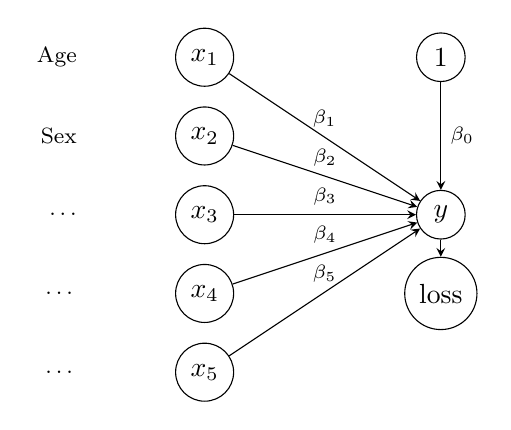
\begin{tikzpicture}[
		  % Define the style of the neural network nodes
		  neuron/.style={circle, draw, minimum size=1.5em},
		  % Define the style of the arrow between nodes
		  arrow/.style={->, >=stealth},
		  % Define the style of the weights
		  weight/.style={midway, above, font=\scriptsize},
		  % Define the style of the input labels
		  inputlabel/.style={above, font=\small},
		  % Define the style of the informative text labels
		  infolabel/.style={left, font=\footnotesize, align=center}
		  ]

		  % Input layer nodes
		  \foreach \i/\info in {1/Age, 2/Sex, 3/$\ldots$, 4/\ldots, 5/\ldots} {
		    \node[neuron] (input\i) at (0, -\i) {$x_{\i}$};
		    \node[infolabel] at (-1.5, -\i) {\info};
		  }
		  % intercept node
		  \node[neuron] (intercept) at (3, -1) {$1$};

		  % Output node
		  \node[neuron] (output) at (3, -3) {$y$};
		  \node[neuron, below of=output] (loss) {loss};

		  % Connect the nodes
		  \foreach \i in {1, ..., 5} {
		    \draw[arrow] (input\i) -- (output) node[weight] {$\beta_{\i}$};
		  }
		  \draw[arrow] (intercept) -- (output) node[weight, pos=0.5, right] {$\beta_0$};
		  \draw[arrow] (output) -- (loss) node[weight, midway, above] {};
    \end{tikzpicture}
\end{figure}

\begin{figure}
    \centering
    \tikzsetnextfilename{neural-network}
		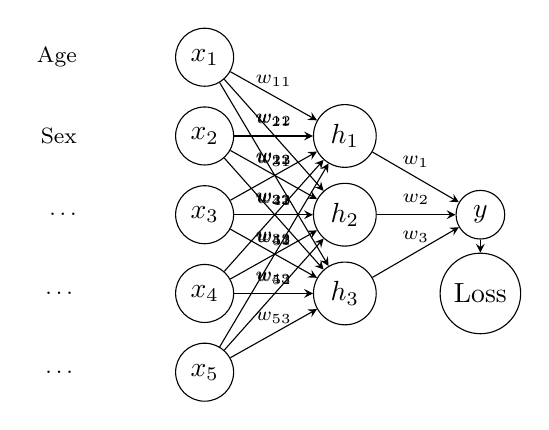
\begin{tikzpicture}[
		  % Define the style of the neural network nodes
		  neuron/.style={circle, draw, minimum size=1.5em},
		  % Define the style of the arrow between nodes
		  arrow/.style={->, >=stealth},
		  % Define the style of the weights
		  weight/.style={midway, above, font=\scriptsize},
		  % Define the style of the input labels
		  inputlabel/.style={above, font=\small},
		  % Define the style of the informative text labels
		  infolabel/.style={left, font=\footnotesize, align=center}
		  ]

		  % Input layer nodes
		  \foreach \i/\info in {1/Age, 2/Sex, 3/$\ldots$, 4/\ldots, 5/\ldots} {
		    \node[neuron] (input\i) at (0, -\i) {$x_{\i}$};
		    \node[infolabel] at (-1.5, -\i) {\info};
		  }

		  % Hidden layer nodes
		  \foreach \h [evaluate=\h as \k using {\h + 1}]in {1, 2, 3} {
		    \node[neuron, right=1cm of input\k] (hidden\h) {$h_{\h}$};
		  }

		  % Output node
		  \node[neuron, right=1cm of hidden2] (output) {$y$};
		  \node[neuron, below of=output] (loss) {Loss};

		  % Connect the nodes
		  \foreach \i in {1, ..., 5} {
		    \foreach \h in {1, 2, 3} {
		      \draw[arrow] (input\i) -- (hidden\h) node[weight] {$w_{\i\h}$};
		    }
		  }
		  \foreach \h in {1, 2, 3} {
		    \draw[arrow] (hidden\h) -- (output) node[weight] {$w_{\h}$};
		  }
		  \draw[arrow] (output) -- (loss) node[weight, midway, above] {};
		\end{tikzpicture}
\end{figure}

\end{document}
